\documentclass[../00_main.tex]{subfiles}

\begin{document}

\section{Python Satellite Data Program}

This section details how to set up and use the program. First, the setup is 
discussed and then each of the successive stages is detailed.\\

The information about library functions and ways to use Python and the 
libraries are taken from the respective documentation. Because many different
libraries and elements work together, I will not go into detail for every 
single one but list the required ones and a quick description in Table
\ref{tab:01}. They are listed in no particular order.
\begin{table}[H]
    \center
\begin{tabular}{| l | l | l |}\hline
    Name        & Reference         & Purpose       \\\hline\hline
    PyQt5       & \cite{pyqt}       & creation of GUI, handling of threading
                                        \\\hline
    os          & \cite{py-os}      & creating and checking directories
                                        \\\hline
    numpy       & \cite{py-numpy}   & managing data and manipulating arrays
                                        \\\hline
    pandas      & \cite{pandas}     & exporting data, providing data to plot, 
                                        creating date series\\\hline
    json        & \cite{py-json}    & reading and writing JSON files
                                        \\\hline
    datetime    & \cite{py-datetime}& date objects, converting dates, 
                                        difference between dates\\\hline
    textwrap    & \cite{py-textwrap}& wrapping text at $n$ characters for 
                                        titles\\\hline
    math        & \cite{py-math}    & testing for NaN
                                        \\\hline
    cartopy     & \cite{py-cartopy} & creation of maps, borders, transforming 
                                        maps\\\hline
    matplotlib  & \cite{py-mpl}     & creating plots, saving plots to files
                                        \\\hline
    netCDF4     & \cite{netcdf4}    & reading netCDF files
                                        \\\hline
    pathlib     & \cite{pathlib}    & working with file paths, getting current 
                                        path\\\hline
    re          & \cite{py-re}      & regular expressions to modify file names
                                        \\\hline
    webbrowser  & \cite{browser}    & library to open a web page in a local 
                                        browser\\\hline
    sys         & \cite{py-sys}     & required to pass system arguments to 
                                        PyQt5\\\hline
    warnings    & \cite{warnings}   & ignoring warnings from netCDF4 that I 
                                        cannot control\\\hline
\end{tabular}
    \caption{Table of required libraries}
    \label{tab:01}
\end{table}

\subsection{Setup}

The programs and data required to use the program are the following:
\begin{itemize}
    \item netCDF data files (preferably from M2I3NPASM because it has been
        tested),
    \item a working installation of the Anaconda Python distribution (available
        \href{https://www.anaconda.com/products/individual}{here}),
    \item download the code for my program from my Github repository 
        \href{https://github.com/moritz-konarski/internship}{here} or request
        it from me.
\end{itemize}
Now an Anaconda environment which is required to run the program needs to be
created. Setting up the Anaconda environment is simple. Navigate to the 
"programs" folder in the downloaded folder of my code. Then, open that folder 
in a terminal. Any UNIX terminal should work, but it must be cmd.exe on 
Windows, Powershell will not work without some modifications. In the terminal, 
type\\
\texttt{conda env create --file internship\_gui.yml}\\
\noindent
On Windows, use\\
\texttt{conda env create --file internship\_gui\_win.yml}\\
\noindent
This command will create an Anaconda Python environment with all the required 
dependencies and libraries for my program. The installation might take a while. 
The resulting environment will have the same name as the file it was created 
from. To use the environment it has to be activated with\\
\texttt{conda activate internship\_gui} \\
\noindent
or \\
\texttt{conda activate internship\_gui\_win}\\
\noindent
on Windows. Once the environment is activated, navigate to the "gui\_program" 
folder. To execute the program, run the command\\
\texttt{python3 main.py}\\
\noindent
or on Windows:\\
\texttt{python main.py}\\
\noindent
If you see a window that looks like \figref{dp01}, the installation and setup 
was successful!

\subsection{Data Processing}

\begin{figure}[H]
    \center
    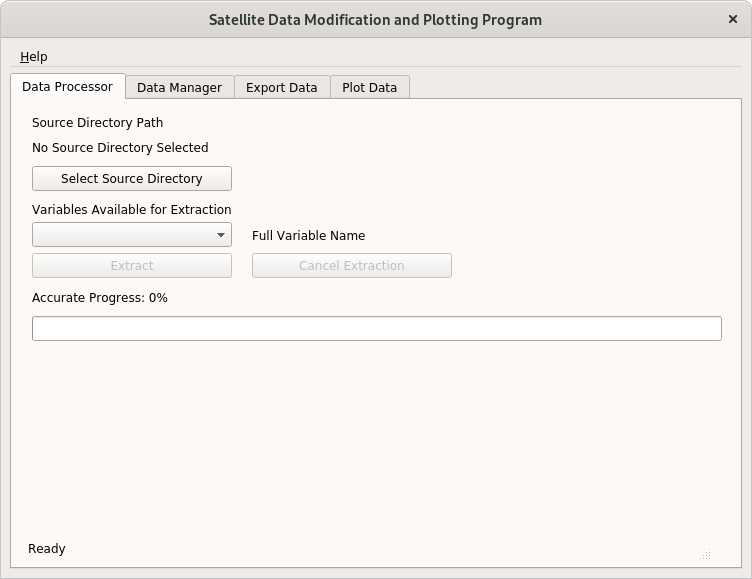
\includegraphics[width=0.75\textwidth]{../graphics/dp01}
    \caption{The Data Processor Tab}
    \label{dp01}
\end{figure}
The first screen of the program is the Data Processor as seen in \figref{dp01}.
The purpose of the Data Processor is to take netCDF files as input, extract
a single variable from them and save it to an NPZ file. It is made up of two
classes, the DataProcessor class, a QThread that performs the processing, and 
the DataProcessorTab class which handles the UI. The steps to using it are the 
following:
\begin{enumerate}
    \item Click the \textbf{Select Source Directory} button. An input dialog
        (\figref{dp02}) will appear where you will have to select the folder 
        where the netCDF files are located. The validity of the specified 
        directory will be checked. 
            \begin{figure}[H]
                \center
                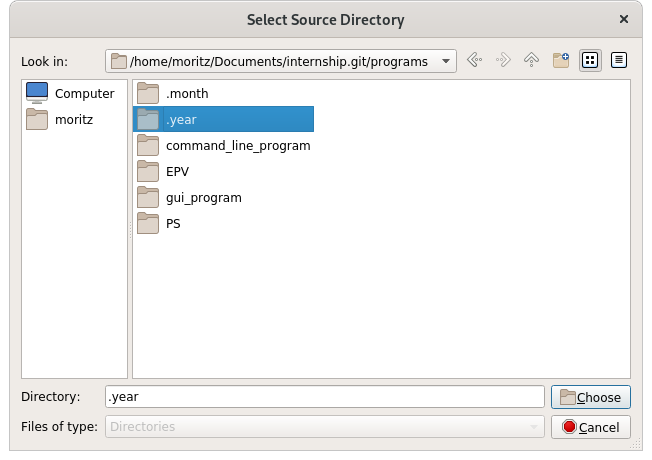
\includegraphics[width=0.75\textwidth]{../graphics/dp02}
                \caption{The Source Directory Selection Popup}
                \label{dp02}
            \end{figure}
    \item After \textbf{Choose} is clicked, the directory is checked to
        make sure it contains netCDF files. Then, the available variables are 
        extracted from the first file. They are displayed in a drop--down list 
        in their short form and then the selected one's full name is displayed 
        (see \figref{dp03}). Here the user must choose one of the variables to 
        extract. 
        \begin{figure}[H]
            \center
            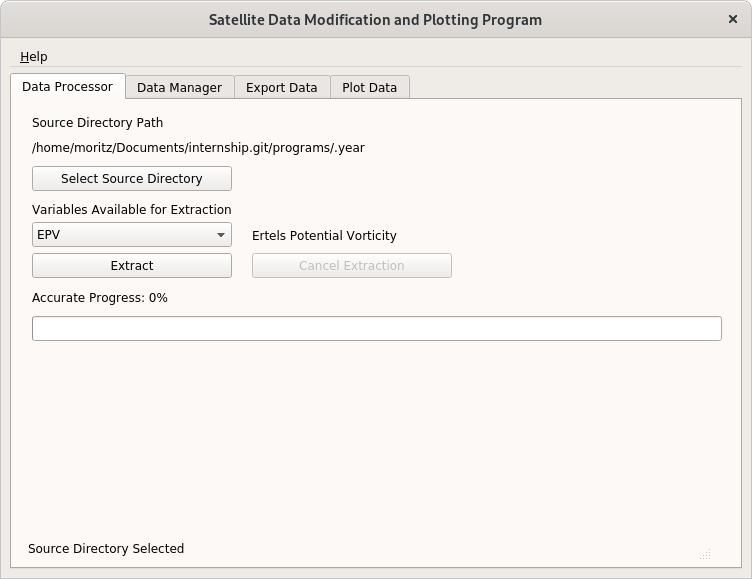
\includegraphics[width=0.75\textwidth]{../graphics/dp03}
            \caption{Data Processor with loaded source Directory}
            \label{dp03}
        \end{figure}
    \item When the choice is made, click \textbf{Extract}. A popup asking
        for a destination directory will appear where the user should
        indicate where the files should be saved. In case the extraction
        takes too long or the user changes their mind, the \textbf{Cancel
        Extraction} button will stop the extraction process. \figref{dp04}
        shows the extraction process.
        \begin{figure}[H]
            \center
            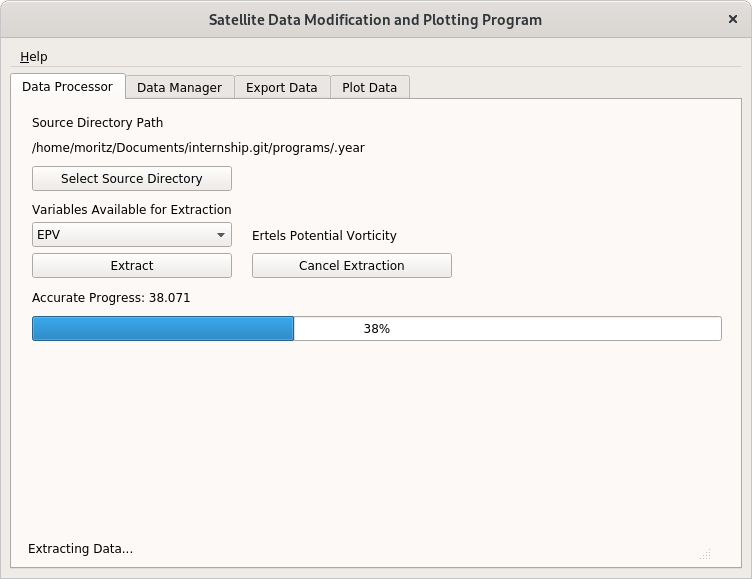
\includegraphics[width=0.75\textwidth]{../graphics/dp04}
            \caption{Extraction in Progress}
            \label{dp04}
        \end{figure}
\end{enumerate}
This process will create a new directory in the directory the user selected.
It will be named after the short name of the variable and contain the NPZ file 
named <short variable name>.npz. That file will contain all the relevant data. 
Furthermore, it will contain a file called metadata.json, which contains all 
the important metadata information that was contained in the netCDF file.
\newline

Once the extraction process is complete, the user can either continue using
this program and switch to the Data Manager tab, or take the created folder and
use the NPZ file with any NumPy--compatible program.

\subsection{Data Management}

\begin{figure}[H]
    \center
    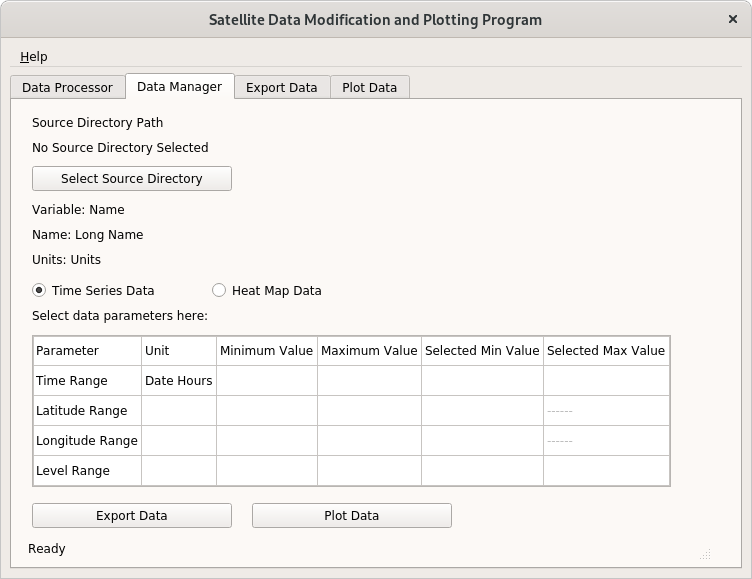
\includegraphics[width=0.75\textwidth]{../graphics/dm01}
    \caption{The Data Manager Tab}
    \label{dm01}
\end{figure}

The Data Manager seen in \figref{dm01} is responsible for selecting the data 
subset the user intends to use and the type of data the user intends to use.
The data subset is defined by setting minimum and maximum values for the
dimensions of the data. The type of data is either a time series, where
a location is fixed and all data for that point is available, or a heat map
where a range of latitude and longitude is selected and then all data for that
selection is used. The Data Manager, much like the Data Processor, has two
parts, the DataManager, responsible for providing the data, and the
DataManagerTab, which is responsible for the GUI. The Data Manager is used like 
this:
\begin{enumerate}
    \item Click the \textbf{Select Source Directory} button. An input dialog
        (like \figref{dp02}) will appear where you will have to select the 
        folder that was created by the Data Processor (the validity of the 
        folder will be checked).
    \item After the directory has been successfully selected, the variable
        name, long variable name, and the unit of the variable will be
        displayed. Furthermore, the table at the bottom will be filled in with
        the minimum and maximum values that are available according to the file
        that was provided. \figref{dm02} illustrates this step.
        \begin{figure}[H]
            \center
            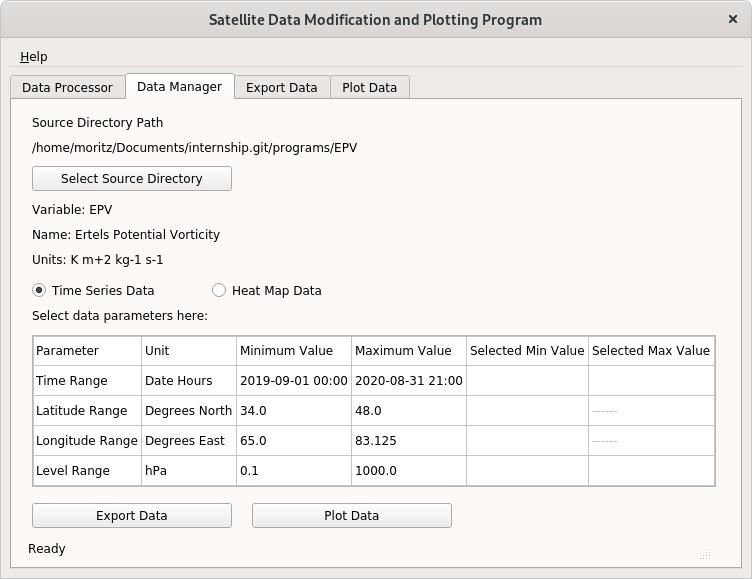
\includegraphics[width=0.75\textwidth]{../graphics/dm02}
            \caption{Data Manager with loaded Directory}
            \label{dm02}
        \end{figure}
    \item With the directory selected, the user now needs to choose the limits
        of the data dimensions by entering them into the table. All user input 
        will be validated and in case a value is outside of the possible 
        values, an error message is shown. Furthermore, all entered values will
        automatically be corrected to the closest available value. \\
        The radio buttons determine if time series data (see \figref{dm03}) or 
        heat map data (see \figref{dm04}) is selected and the table is adjusted 
        accordingly. If the selected data does not have a level associated with 
        it, the last row of the table is disabled (see \figref{dm05}).
        \begin{figure}[H]
            \center
            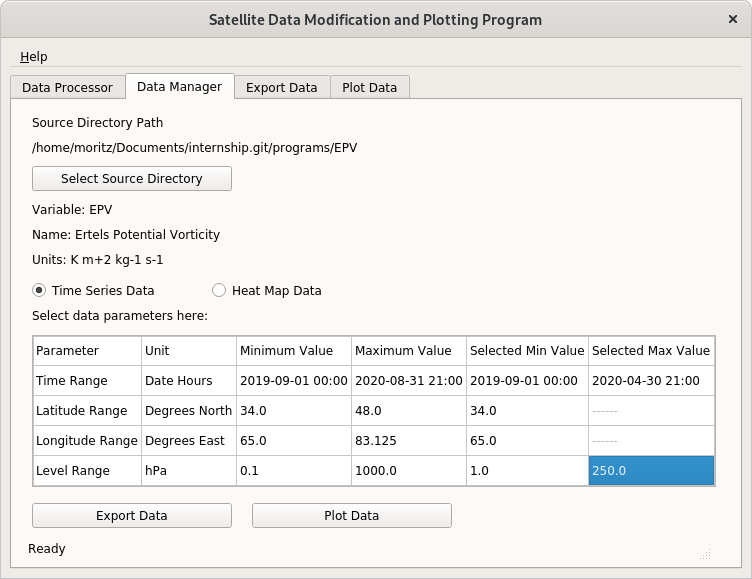
\includegraphics[width=0.75\textwidth]{../graphics/dm03}
            \caption{Data Manager in Time Series Mode}
            \label{dm03}
        \end{figure}
        \begin{figure}[H]
            \center
            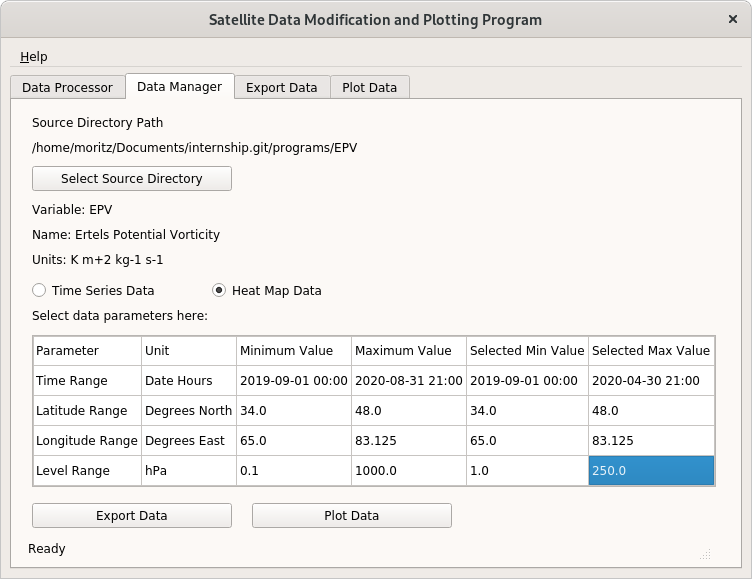
\includegraphics[width=0.75\textwidth]{../graphics/dm04}
            \caption{Data Manager in Heat Map Mode}
            \label{dm04}
        \end{figure}
        \begin{figure}[H]
            \center
            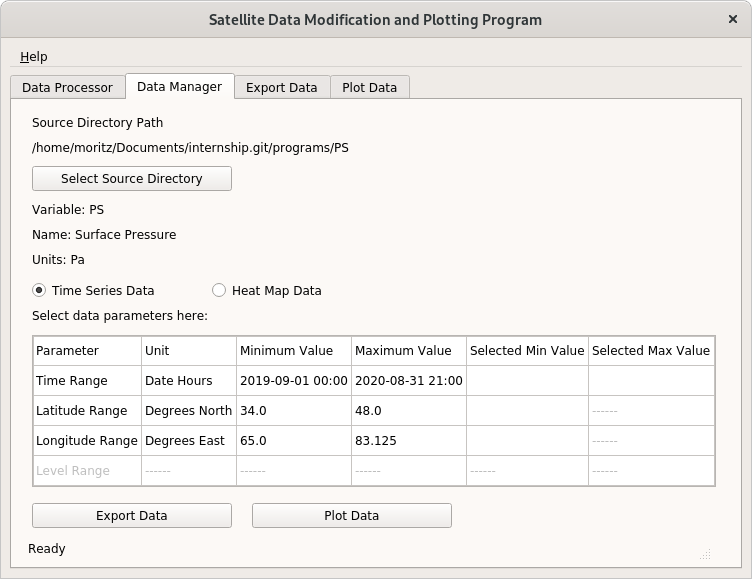
\includegraphics[width=0.75\textwidth]{../graphics/dm05}
            \caption{Data Manager with data without level}
            \label{dm05}
        \end{figure}
    \item When all data fields have been filled, the user may either press the
        \textbf{Export Data} button or the \textbf{Plot Data} button. Each of
        the buttons will prepare the associated data and then switch to the
        corresponding tab.
\end{enumerate}
The values entered in the Data Manager are persistent, meaning that if the user
exports some data first and then wants to plot the same data, they only need to
go back to the Data Manager tab and press \textbf{Plot Data}.

\subsection{Data Exporting}

\begin{figure}[H]
    \center
    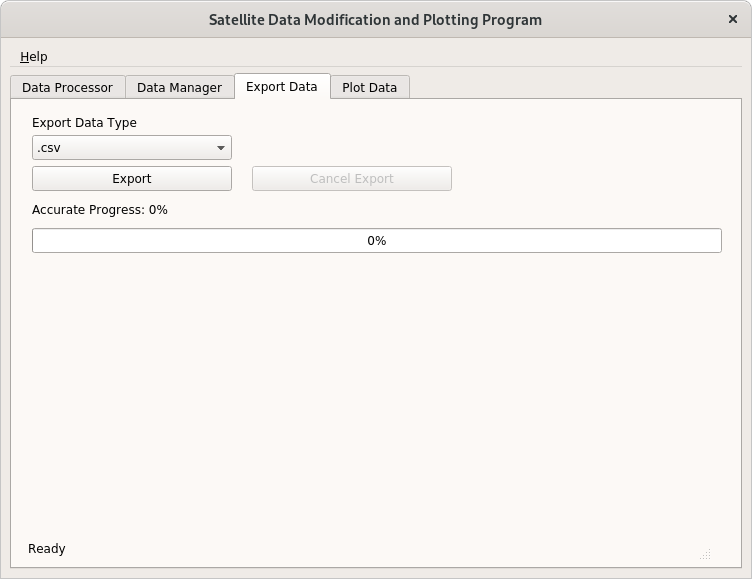
\includegraphics[width=0.75\textwidth]{../graphics/de01}
    \caption{The Data Export Tab}
    \label{de01}
\end{figure}

If the user pressed the \textbf{Export Data} button, they will be taken to the
Export Data tab. Again, this tab's functionality is coded in the DataExporter 
class and the GUI is in the DataExporterTab class. \figref{de01} shows what the 
user sees. To use the data manager, the following actions are required:
\begin{enumerate}
    \item The user is required to choose one of the 4 options of export data
        types from the drop--down list seen in \figref{de01}. The available
        options are ".cvs" (comma separated values), ".zip" (compressed file), 
        ".xlsx" (an MS Excel file), or ".html" (a website file to be opened in 
        the browser). 
    \item After making their choice, the user needs to press the
        \textbf{Export} button to begin the export process. Because this
        process might produce 1000s of files depending on the data settings
        specified, the program will give the user a warning about the number of
        files that will be created (see \figref{de02}). 
        \begin{figure}[H]
            \center
            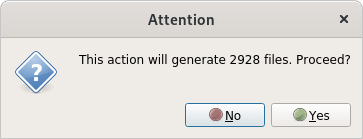
\includegraphics[width=0.5\textwidth]{../graphics/de02}
            \caption{The File Number Warning Message}
            \label{de02}
        \end{figure}
        If the user clicks \textbf{Yes}, the
        export begins. Then, the program will ask for a destination directory 
        where the files will be saved in a new directory called "<variable
        name>-exported". If the process takes too long or the user simply wants 
        to interrupt it, they need to press the \textbf{Cancel Export} button. 
        The progress bar will show the extraction progress as illustrated by 
        \figref{de03}
        \begin{figure}[H]
            \center
            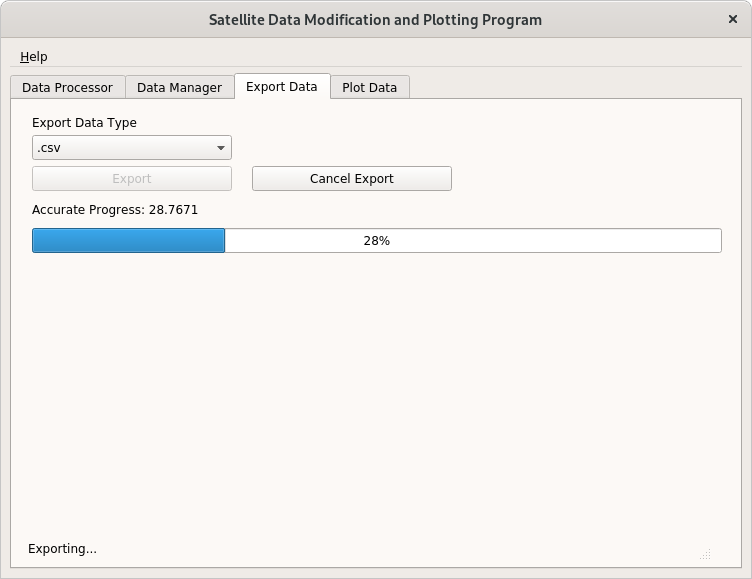
\includegraphics[width=0.75\textwidth]{../graphics/de03}
            \caption{Data Export in progress}
            \label{de03}
        \end{figure}
\end{enumerate}
When heat map data is being exported, a file will be created for each time step
and for each level in each time step. This may lead to a large number of
files -- which the warning message (\figref{de02}) is meant for.\\

When time--series data is being exported, a file will be generated for each
level but because time--series cover multiple time values, all selected time 
values will be in one file. This leads to a manageable number of files.\\

The exported files will be saved in files with the following file names:
\begin{itemize}
    \item \textbf{Heat Map}: "Heat Map <long variable name> <date and
        time> <minimum latitude and longitude values>-<maximum latitude and
        longitude values> <pressure level>.<file type>" (the pressure will be
        omitted if the data does not include it).\\
        An example of this type of file name is "Heat Map Ertels Potential 
        Vorticity 2019-09-01 00:00 (34.0N, 65.0E)-(48.0N, 83.125E) 1.0 hPa".
    \item \textbf{Time--series}: "Time Series <long variable name>
        <start date and time>-<end date and time> <latitude and longitude> 
        <pressure level>.<file type>" (the pressure will be
        omitted if the data does not include it).\\
        An example of this type of file name is "Time Series Ertels Potential 
        Vorticity 2019-09-01 00:00-2019-09-10 00:00 (34.0N, 65.0E) 1.0 hPa".
\end{itemize}
To demonstrate the result see Table \ref{tab:de01} which contains the exported
data for air temperature T in Kelvin at a pressure of 250 hPa at 
34\textdegree{}N, 65\textdegree{}E from 01.09.2019 00:00 to 30.09.2019 21:00. 
The data has been cut off to save space.
\begin{table}[H]
\center
    \begin{tabular}{| p{5cm} | p{5cm} |} \hline
        2019-09-01 00:00:00   &  237.30182  \\\hline 
        2019-09-01 03:00:00   &  236.86859  \\\hline
        2019-09-01 06:00:00   &  236.79724  \\\hline
        2019-09-01 09:00:00   &  236.82132  \\\hline
        2019-09-01 12:00:00   &  237.73062  \\\hline
        2019-09-01 15:00:00   &  238.40472  \\\hline
        2019-09-01 18:00:00   &  238.4401   \\\hline
        2019-09-01 21:00:00   &  238.20715  \\\hline
        2019-09-02 00:00:00   &  237.49396  \\\hline
    \end{tabular}
    \caption{Temperature \texttt{T} exported as \texttt{.csv}}
    \label{tab:de01}
\end{table}

\subsection{Data Plotting}

\begin{figure}[H]
    \center
    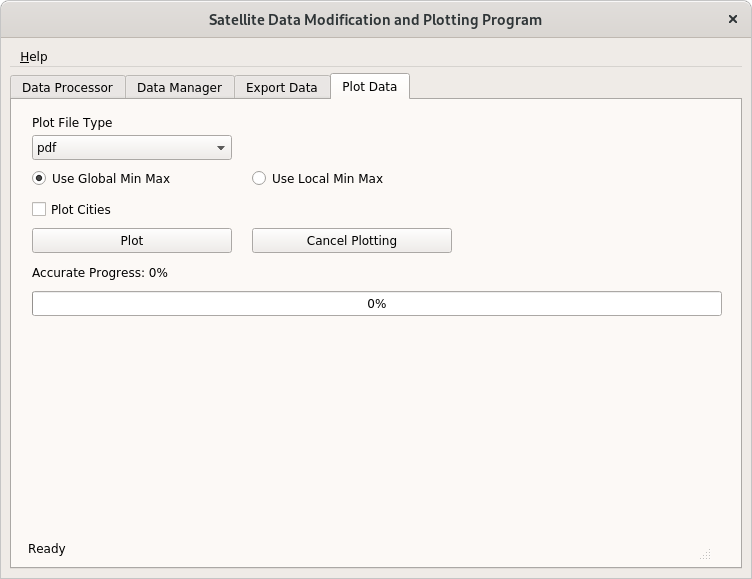
\includegraphics[width=0.75\textwidth]{../graphics/dpl01}
    \caption{The Data Plotter Tab for Heat Map Data}
    \label{dpl01}
\end{figure}

If the user chooses to push the \textbf{Plot Data} button in the Data Manager
tab, they will be shown the Data Plot tab. As with all other tabs, the UI is
handled by a class called DataPlotterTab, and the plotting itself is handled by 
the DataPlotter. The GUI the user will see if they chose to plot heat map data 
is illustrated in \figref{dpl01}. If the user chose time series data, 
\figref{dpl02} will be shown (the \textbf{Plot Cities} check box will be 
disabled). 
\begin{figure}[H]
    \center
    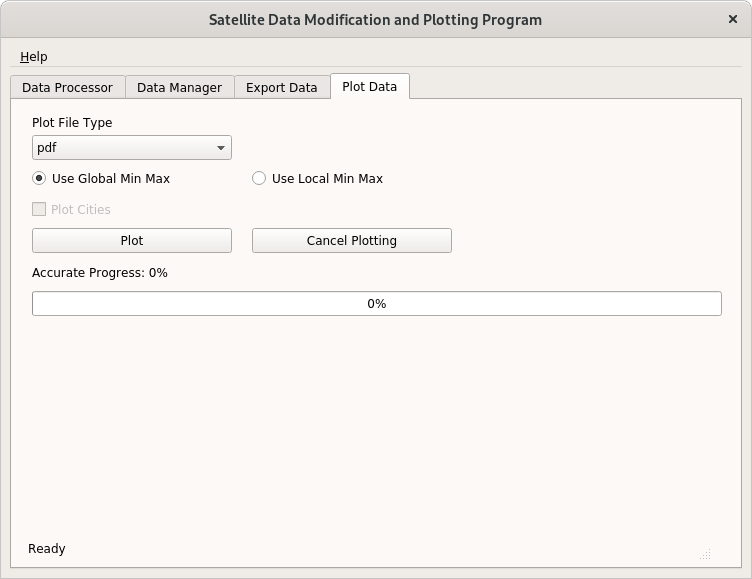
\includegraphics[width=0.75\textwidth]{../graphics/dpl02}
    \caption{The Data Plotter Tab for Time Series Data}
    \label{dpl02}
\end{figure}
The steps to using this tab are very similar to the Data
Exporter tab; they are:
\begin{enumerate}
    \item The user chooses one of the 5 options of plot data
        types from the drop--down list seen in \figref{dpl01}. The available
        options are ".pdf" (portable document format), ".png" (portable network 
        graphics), ".eps" (encapsulated PostScript), ".svg" (scalable vector 
        graphics), or ".jpeg". 
    \item The next option is whether or not to use global minima and maxima or
        to use local minima and maxima. Using global minima and maxima means
        that if the user selected a range of 2 days, the minimum and maximum 
        values of all measurements in these 2 days are used as the axis limits.
        If the user chooses local minima and maxima, the minimum and maximum
        value for each plot will be used. The former makes is easier
        to compare multiple plots with each other, while the latter creates
        more fitting individual plots.
    \item If the user is plotting heat map data they can choose whether or not
        to plot cities on their heat map. The cities that will be plotted are
        Bishkek, Almaty, Kabul, Tashkent, and Dushanbe.
    \item After making these choices, the user needs to press the
        \textbf{Plot} button to begin the plotting process. This
        process might produce 1000s of files depending on the data settings
        specified, so the program will give the user a warning about the number 
        of files that will be created (see \figref{de02} above).\\
        If the user clicks \textbf{Yes}, the export begins. Then, the program 
        will ask for a destination directory where the files will be saved in a 
        new directory called "<variable name>-plotted". If the process takes 
        too long or the user simply wants to interrupt it, they need to press 
        the \textbf{Cancel Plotting} button. The progress bar will show the
        extraction progress as illustrated by \figref{de03}
        \begin{figure}[H]
            \center
            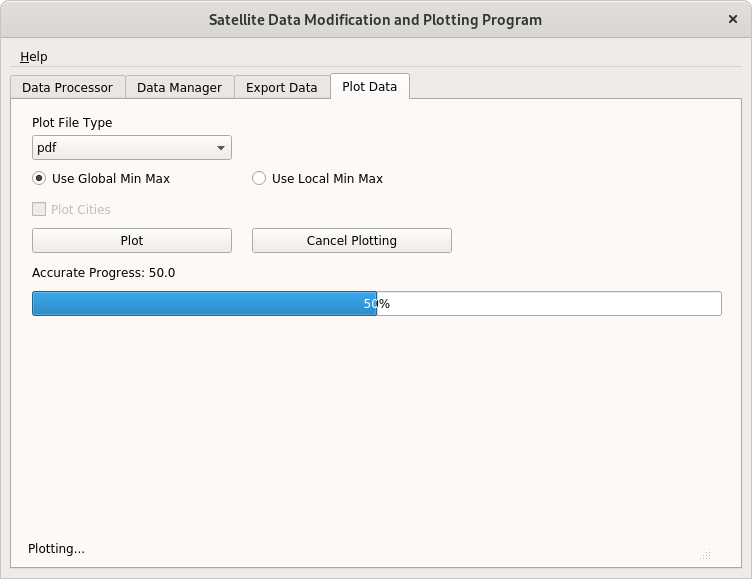
\includegraphics[width=0.75\textwidth]{../graphics/dpl03}
            \caption{Data Plotter in Progress}
            \label{dpl03}
        \end{figure}
\end{enumerate}
When heat map data is being exported, a file will be created for each time step
and for each level in each time step unless the plot data type is PDF. If PDF
is chosen all the plots will be put into one large PDF file with a page for
each of the plots. If PDF is not the file type, a large number of
files may be generated.\newline

When time--series data is being plotted, a file will be generated for each
level but because time series contain multiple time steps, all selected time 
values will be in one file. This leads to a manageable number of
files.\\
The exported files will be saved in files with the same files names as
specified in the Data Export section above.\newline

Sticking with the temperature example from above, the time series plot of the
same data that is shown in \figref{tab:de01} is plotted in \figref{plt:dpl01}.
The $y$ axis shows the temperature in Kelvin ($K$) and the $x$ axis shows the
date and time of the measurement.
\begin{figure}[h]
    \center
    \fbox{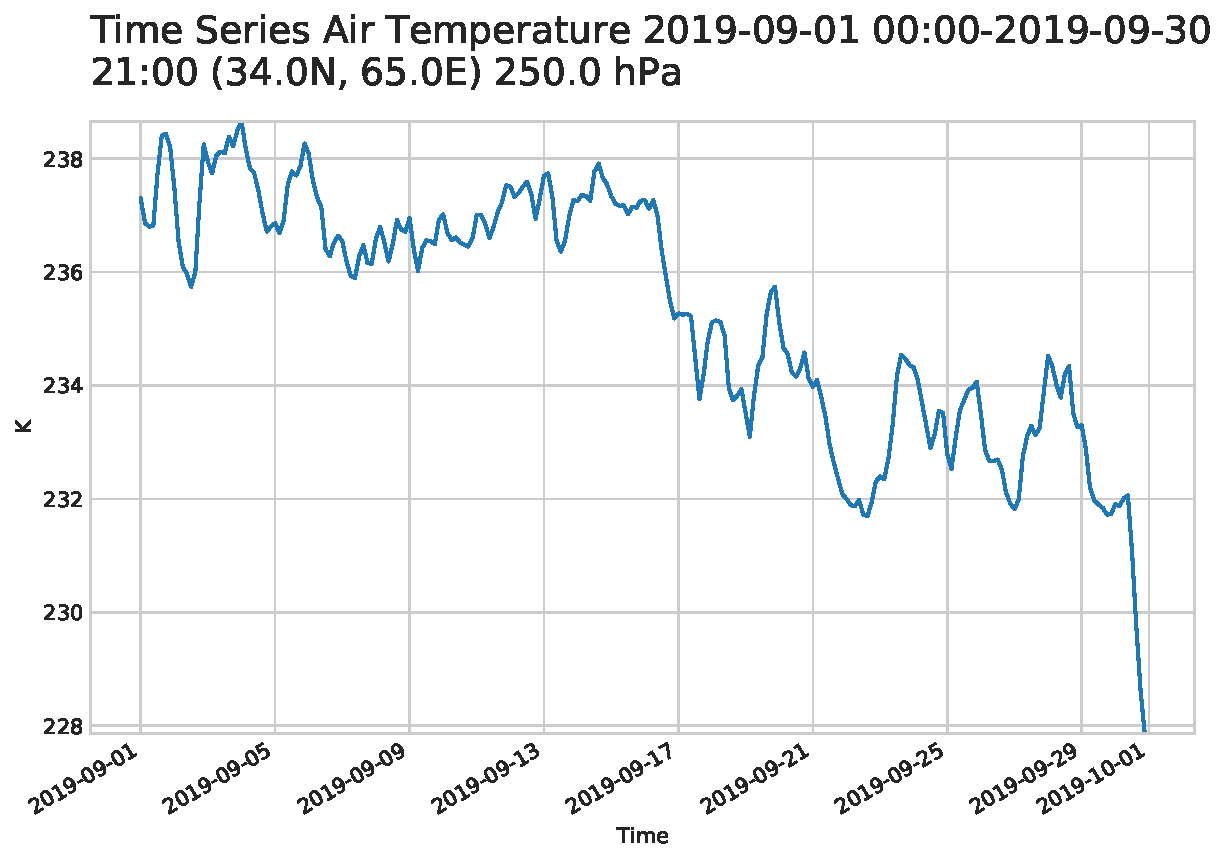
\includegraphics[width=0.9\textwidth]{../graphics/plt01}}
    \caption{Time Series Plot for Air temperature}
    \label{plt:dpl01}
\end{figure}
In \figref{plt:dpl02} a heat map of the air temperature on 01.09.2019 at 00:00
at a pressure of 250 hPa is graphed for a region from (34\textdegree{}N,
65\textdegree{}E) to (48\textdegree{}N, 83.125\textdegree{}E).\\
Here the $x$ and
$y$ axes show the latitude and longitude, respectively and the temperature is
indicated by the contour. The temperatures corresponding to the colors can be
seen in the color bar to the right (also in Kelvin $K$).
\begin{figure}[H]
    \center
    \fbox{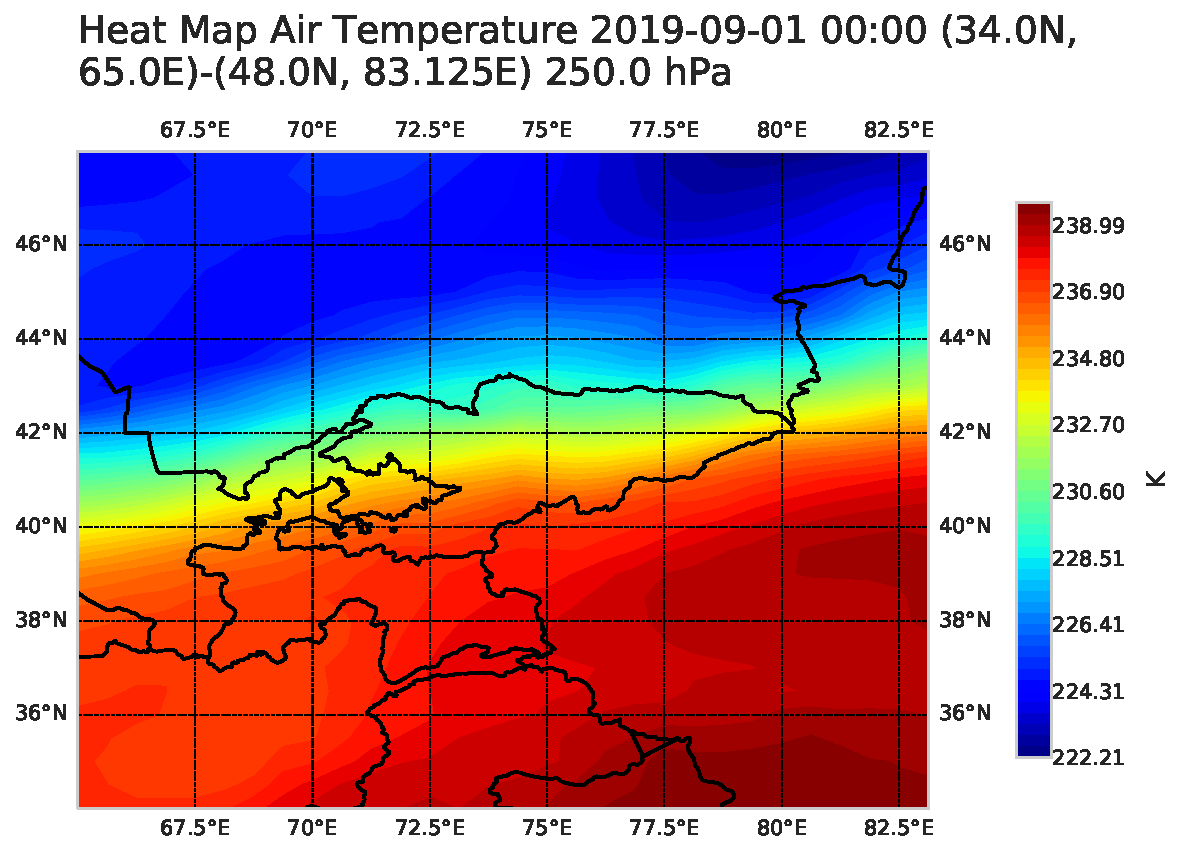
\includegraphics[width=0.9\textwidth]{../graphics/plt02}}
    \caption{Heat Map Plot for Air temperature}
    \label{plt:dpl02}
\end{figure}
\figref{plt:dpl03} shows the same plot as \figref{plt:dpl02}, but with city
plotting enabled.
\begin{figure}[h]
    \center
    \fbox{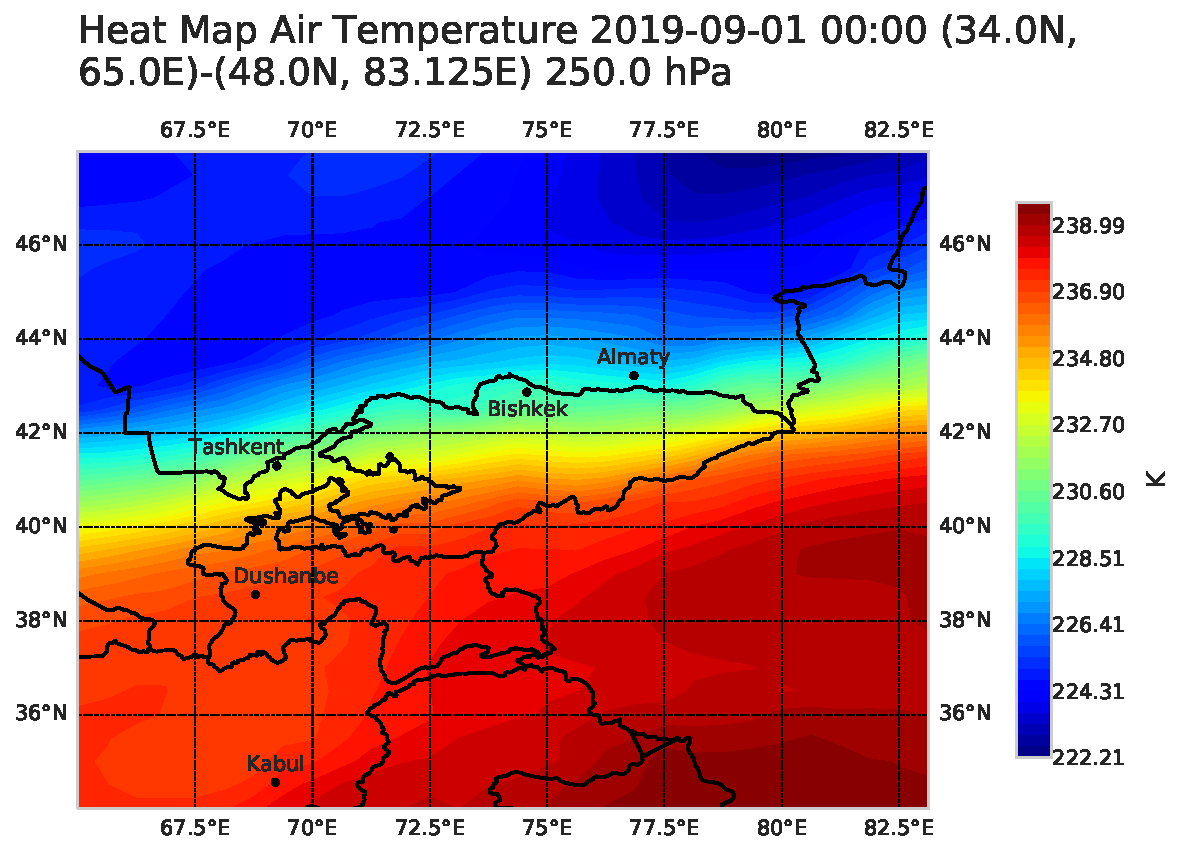
\includegraphics[width=0.9\textwidth]{../graphics/plt03}}
    \caption{Heat Map Plot for Air Temperature with cities}
    \label{plt:dpl03}
\end{figure}

\subsection{Help}

The last and maybe most important section of the program is the help section.
It can be accessed by clicking on the text \textbf{Help} in the menu bar at the
top of the program window as seen in every figure of the program window, e.g.
\figref{dpl03}. This will open a local HTML file in a browser tab.\newline

This website is based on a template given to me by my supervisor to create the 
help section. It contains a table of contents, a short introduction to what the
program does, and then a short description of what each of the 4 tabs does,
similar to the one provided in this section. In \figref{help} the menu and
introduction are shown as they appear in a browser.
\begin{figure}[H]
    \center
    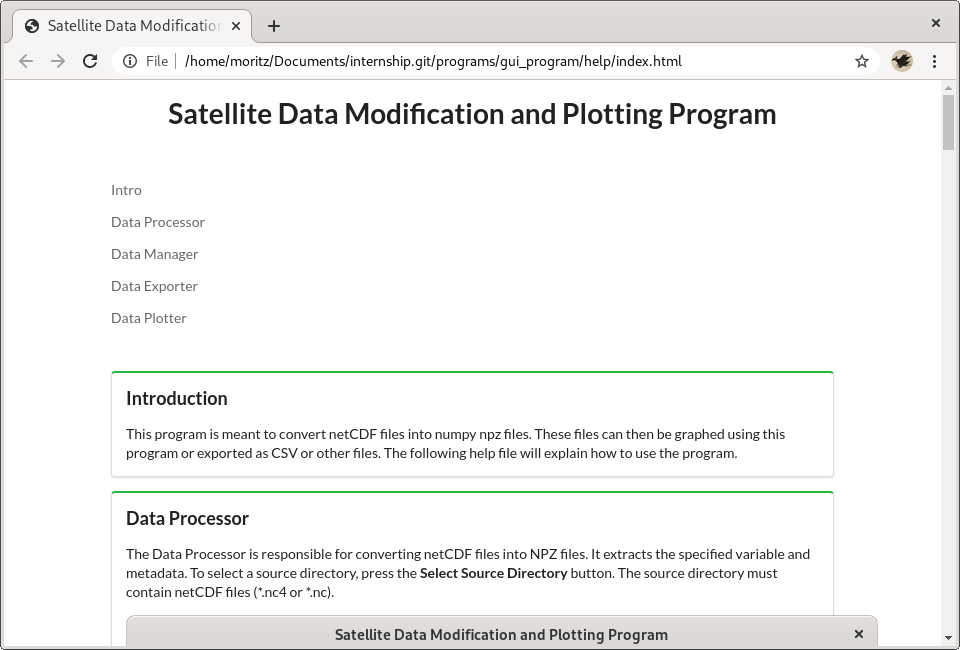
\includegraphics[width=\textwidth]{../graphics/help}
    \vspace{-20pt}
    \caption{Screen Shot the Help section}
    \label{help}
\end{figure}

\end{document}
